\chapter{Constructing measures}\label{ch:ch1}\label{measureChapter}
A measure is a rule by which we assign ``size'' to certain sets.
The notion of a measure generalizes a handful of familiar notions, which we now review.
\begin{example}\label{examples of measures}
If $X$ is a set, we will define a measure known as the \dfn{counting measure} $\mu$ of $X$, by declaring that for every finite subset $Y \subseteq X$, $\mu(Y)$ is the cardinality of $Y$ (i.e.\ the number of elements of $Y$).

We define the \dfn{Lebesgue measure}\footnote{Named after Henri Lebesgue (1875--1941), a French mathematician who introduced measure theory in his book \emph{Intégrale, longueur, aire} (\emph{Integral, length, area}).}
$\mu$ on boxes $[a_{1}, b_{1}] \times \cdots \times [a_{d}, b_{d}] \subseteq \RR^{d}$ by declaring that
\[\mu([a_{1}, b_{1}] \times \cdots \times [a_{d}, b_{d}]) = (b_{1} - a_{1})(b_{2} - a_{2})\cdots(b_{d} - a_{d}).\]
When $d = 1$ this is just the familiar notion of the length of a line segment; when $d = 2$ this is the area of a rectangle; when $d = 3$ this is the volume of a rectangular prism.

In probability theory, one is concerned with sets of ``outcomes'', or possible states that the world could be in.
The sets are known as ``events''.
Given an event $E$ in a sample space $X$, we define $\mu(E)$ to be the probability that the state that the world is in lies in $E$. Thus $\mu(X) = 1$.
\end{example}

\section{Algebras of sets}
A measure, remember, is going to be a rule that assigns a size to certain sets.
In other words it will be a function
$$\mu: \Sigma \to [0, \infty]$$
where $\Sigma$ is a set whose elements are subsets of a fixed set $X$.
The first thing we need to do is determine what algebraic properties $\Sigma$ should have.

\begin{subsec}
To motivate the definition of $\Sigma$, we look to probability theory, using the terminology of Example \ref{examples of measures}.
Recall that in probability theory, elements of $X$ are outcomes, or states that the world could be in; suppose that the world is actually in state $x$.
An observer, Alice, might not have enough information to deduce that the world is in state $x$, but given an event $E \subseteq X$, Alice might be able to deduce whether $x \in E$.

Let $\Sigma$ be the set of events $E$ such that Alice knows whether $E \ni x$.
Since \emph{every} outcome is in $X$, $X \in \Sigma$.
Now suppose that $Y, Z \in \Sigma$. Then Alice knows whether $x \in Y,x \in Z$, so she also knows whether $x \in Y \setminus Z$.\footnote{If Alice knows that $x \in Z$, then she knows that $x \notin Y \setminus Z$. Otherwise, she knows that $x \notin Z$, so $x \in Y \setminus Z$ iff $x \in Y$, and Alice knows that $x \in Y$.}
Furthermore, if $Y_1, Y_2, \dots$ is a countable sequence of events, then $x$ lies in their union $\bigcup_n Y_n$ iff there is $n \in \NN$ such that $x \in Y_n$; so if $Y_1, Y_2, \dots \in \Sigma$ then Alice can deduce whether $x \in \bigcup_n Y_n$, thus $\bigcup_n Y_n \in \Sigma$.

Thus, a set $\Sigma \ni X$ of subsets of $X$ which is closed under countable union and complement represents the information that an observer has.
Such sets $\Sigma$ are so important that we give them a special name, as follows.
\end{subsec}

\begin{definition}
A \dfn{$\sigma$-algebra}\footnote{Here $\sigma$ should be thought of as meaning ``countable'', referring to the closure under countable unions.} in a set $X$ is a set $\Sigma$, whose elements are subsets of $X$, such that:
\begin{enumerate}
\item $X \in \Sigma$.
\item If $Y, Z \in \Sigma$ then $Y \setminus Z \in \Sigma$.
\item If $Y_1, Y_2, \dots$ is a countable sequence of sets in $\Sigma$ then $\bigcup_n Y_n$ is in $\Sigma$.
\end{enumerate}
\end{definition}

\begin{subsec}
$\sigma$-algebras have strong closure properties. For example, if $\Sigma$ is a $\sigma$-algebra, then $\emptyset = X \setminus X \in \Sigma$ (Alice knows that an event which is impossible did not happen).
Furthermore, if $Y \in \Sigma$, then $Y^c = X \setminus Y \in \Sigma$ (if Alice knows whether an event $Y$ happened, then she also knows whether the event ``$Y$ did not happen" happened).
So if $Y_1, Y_2, \dots \in \Sigma$, then
$$\bigcap_n Y_n = \left(\bigcup_n Y_n^c\right)^c \in \Sigma$$
(if Alice knows whether $Y_1, Y_2, \dots$ happened, then she knows whether $Y_1$ happened and $Y_2$ happened and $Y_3$ happened and etc.)
\end{subsec}

\begin{subsec}
Let $\Sigma$ be a $\sigma$-algebra.
In proofs it will frequently be useful to replace sequences of sets in $\Sigma$ with sequences of disjoint sets, without leaving $\Sigma$.
The below lemma allows us to accomplish this.
\end{subsec}

\begin{lemma}
Let $\Sigma$ be a $\sigma$-algebra.
Let ${(E_{n})}_{n}$ be a sequence of sets in $\Sigma$. Then there is a sequence of disjoint sets ${(F_{n})}_{n}$ in $\Sigma$ such that $F_{n} \subseteq E_{n}$ and
\[\bigcup_{n=1}^{\infty} E_{n} = \bigcup_{n=1}^{\infty} F_{n}.\]
\end{lemma}
\begin{proof}
Let $F_{1} = E_{1}$ and for $n \geq 2$,
\[F_{n} = E_{n} \setminus \bigcup_{i=1}^{n-1} F_{i}.\]
Then clearly the $F_{n}$ are disjoint and have the same union as the $E_{n}$.
\end{proof}

\begin{lemma}\label{intersection of rings is ring}
The intersection of a nonempty set of $\sigma$-algebras is a $\sigma$-algebra.
\end{lemma}
\begin{proof}
Let $\mathcal R$ be a set of $\sigma$-algebras and let $\Sigma$ be its intersection.
Since $X \in \Gamma$ for every $\Gamma \in \mathcal R$, $X \in \Sigma$.
If $Y_1, Y_2, \dots \in \Sigma$, then $Y_1, Y_2, \dots \in \Gamma$ for every $\Gamma$, so $Y = \bigcup_n Y_n \in \Gamma$ for every $\Gamma$, so $Y \in \Sigma$.
A similar argument works for closure under complements.
\end{proof}

\begin{subsec}
Whenever we refer to a ``smallest'' set $X$ with a property $P$, we mean that for every set $Y$ with property $P$, $X \subseteq Y$.
\end{subsec}

\begin{lemma}
If $\mathcal C$ is a set of subsets of a set $X$, there is a smallest $\sigma$-algebra containing $\mathcal C$.
\end{lemma}
\begin{proof}
The power set $2^{X} = \{Y: Y \subseteq X\}$ is a $\sigma$-algebra (see Exercise \ref{trivial sigma algebras}) such that for every $\Sigma \in \mathcal C$, $\Sigma \subseteq 2^{X}$.
Let $\mathcal R$ be the set of all $\sigma$-algebras $\Gamma$ such that for every $\Sigma \in \mathcal C$, $\Sigma \subseteq \Gamma$; since $2^{X} \in \mathcal R$, $\mathcal R$ is nonempty, and since $\mathcal R \subseteq 2^{2^{X}}$, $\mathcal R$ is a set\footnote{as opposed to a proper class, like the set of all sets is}.

By Lemma~\ref{intersection of rings is ring}, the intersection $R$ of $\mathcal R$ is a $\sigma$-algebra.
But for every $C \in \mathcal C$, $C \in R$ since $C$ is in every element of $\mathcal R$.
Therefore $R$ contains $\mathcal C$.
\end{proof}

\begin{definition}
The smallest $\sigma$-algebra containing every element of a set $\mathcal C$ is called the \dfn{$\sigma$-algebra generated by} $\mathcal C$.
We denote it by $\sigma(\mathcal C)$.
\end{definition}

\begin{subsec}
The advantage of defining a $\sigma$-algebra by referring to its generators is that it is easy to show that every element of the $\sigma$-algebra has a given property.
This is quite easy to prove, as the following lemma shows, but so very useful.
\end{subsec}

\begin{lemma}\label{generators and relations}
Let $X$ be a set, and let $P$ be a property that subsets of $X$ can have.
Assume that $\mathcal C$ is a set whose elements are subsets of $X$, and every element of $\mathcal C$ has property $P$.
If the set of all subsets of $X$ with property $P$ is a $\sigma$-algebra, then every element of $\sigma(\mathcal C)$ has property $P$.
\end{lemma}
\begin{proof}
Let $\Sigma$ be the $\sigma$-algebra of all subsets of $X$ with property $P$.
Then $\Sigma$ contains $\sigma(\mathcal C)$.
\end{proof}

\begin{subsec}
We now come across the most important example of a $\sigma$-algebra.
If the reader is unfamiliar with topological spaces, in the below definition it suffices to take $X = \RR^{d}$, and $\mathcal T$ the set of all unions of open balls in $\RR^{d}$, as this will be the most important case.
\end{subsec}

\begin{definition}
Let $X$ be a topological space.
Let $\mathcal T$ be the topology of $X$, the set of all open subsets of $X$.
We define the \dfn{Borel $\sigma$-algebra}\footnote{Named after Émile Borel (1871--1956), a French probabilist who introduced many of the key ideas of measure theory.}
$\mathcal B$ of $X$ by $\mathcal B = \sigma(\mathcal T)$.
A \dfn{Borel set} in $X$ is an element of $\mathcal B$.
\end{definition}

\begin{subsec}
Let $X$ be a topological space.
It follows from the definition that every open or closed subset of $X$ is Borel, but also that countable unions of complements of countable unions of complements of countable unions of complements of\dots of open sets of $X$ is Borel.
However, some Borel sets can be even more complicated than that.
\end{subsec}

\begin{lemma}
Let $X$ be a topological space.
Assume that $P$ is a property that subsets of $X$ can have, and that every open set has property $P$.
If the set of subsets of $X$ with property $P$ is a $\sigma$-algebra, then every Borel set has property $P$.
\end{lemma}
\begin{proof}
By Lemma~\ref{generators and relations}.
\end{proof}

\begin{subsec}
When is a set Borel? If $X = \NN$, then every set is open and so every set is Borel.
But it is not so obvious how to check whether a subset of $\RR^{d}$ is Borel.
Certainly any set you will ever ``naturally'' encounter is Borel, but not every subset of $\RR^{d}$ is Borel.
\end{subsec}

\begin{theorem}\label{Borel sigma algebra}
There exists a subset of $\RR^{d}$ which is not Borel.
In fact, the set of Borel subsets of $\RR^{d}$ has strictly lower cardinality than the set of all subsets of $\RR^{d}$.
\end{theorem}
\begin{proof}
We defer the proof to a later stage -- namely, Theorem~\ref{Borel not Lebesgue}.
\end{proof}

\begin{exercise}
Interpret all of the theorems in this section in terms of knowledge that Alice may have.
\end{exercise}

\begin{exercise}\label{trivial sigma algebras}
Let $X$ be a set.
Show that the power set $2^{X}$ --- that is, the set of all subsets of $X$ --- is a $\sigma$-algebra, as is $\{\emptyset, X\}$.
\end{exercise}

\begin{exercise}\label{sigma algebras are rings}
Recall from your algebra class the definition of a ring: a set equipped with an addition and a multiplication satisfying certain axioms.
Show that every $\sigma$-algebra is a ring, where addition and multiplication are replaced by symmetric difference and intersection, respectively.
\end{exercise}

\begin{exercise}
Let $\Sigma$ be an infinite $\sigma$-algebra. Show that $\Sigma$ has cardinality at least that of $2^{\NN}$, the power set of the natural numbers.
(Hint: let $\Sigma_{0} = \Sigma$. Choose $X_{n} \in \Sigma_{n}$ appropriately and let $\Sigma_{n+1} = \{Y \in \Sigma_{n}: X_{n} \cap Y = \emptyset\}$. If done correctly, you should be able to find an injective function $F: 2^{\NN} \to \Sigma$ such that $F(\{n\}) = X_{n}$).
\end{exercise}

\begin{exercise}\label{generators of Borel}
Show that the set of half-open intervals $[a, b)$ generates the Borel $\sigma$-algebra of $\RR$.
\end{exercise}

\begin{exercise}
Show that the set of compact subsets of $\RR^{d}$ generates the Borel $\sigma$-algebra of $\RR^{d}$.
Show that there exists a metric space $X$, such that the set of compact subsets of $X$ does not generate the Borel $\sigma$-algebra of $X$. (Hint: Cardinality!)
\end{exercise}

\begin{exercise}\label{Jordan content 1}
Let us say that a bounded subset $A$ of $\RR$ has \dfn{Jordan content} if the indicator function $1_{A}$ of $A$ is Riemann integrable.
Here $1_{A}(x) = 1$ if $x \in A$ and $1_{A}(x) = 0$ otherwise.
Show that $\QQ$ is Borel, but does not have Jordan content.
Later we will show that every set with Jordan content is Borel, and that it is reasonable to define the length of any Borel set.
So our definitions will generalize those that one learned in a first course in real analysis.
\end{exercise}


\section{The definition of a measure}
We are almost ready to define a measure.
Throughout this section, the reader should refer back to Example~\ref{examples of measures} frequently, as the point of the definitions in this section is to generalize those concepts.

\begin{subsec}
Let $(-\infty, \infty]$ denote the set of real numbers, plus another point $\infty$ which is greater than any real number.
We define addition on $[0, \infty]$ by requiring that $\infty + a = \infty$ for any $a \in \RR$.
We do not define addition on $[-\infty, \infty]$, which would include $-\infty$, because the expression $\infty - \infty$ makes no sense.
\end{subsec}

%\begin{definition}
%Let $B$ be a Banach space or $(-\infty, \infty]$, and let $\mathcal C$ be a collection of sets
%We say that a function $\mu: \mathcal C \to B$ such that for every disjoint sequence of sets ${(X_{n})}_{n}$ in $\Sigma$ such that $\bigcup_{n} X_{n} %\in \mathcal C$,
%\[\mu\bigcup_{n} X_{n} = \sum_{n=1}^{\infty} \mu(X_{n}),\]
%is called a \dfn{$\sigma$-additive fuction}.
%\end{definition}
%Here the infinite sum is meant in the sense of (\ref{banach space series}) if $B$ is a Banach space.

\begin{definition}
Let $\mathcal C$ be a collection of sets.
A function $\mu: \mathcal C \to [0, \infty]$ such that for every disjoint sequence of sets ${(X_{n})}_{n}$ in $\Sigma$ such that $\bigcup_{n} X_{n} \in \mathcal C$,
\[\mu\bigcup_{n} X_{n} = \sum_{n=1}^{\infty} \mu(X_{n}),\]
is called a \dfn{$\sigma$-additive fuction}.
\end{definition}

\begin{definition}
A \dfn{measure} is a $\sigma$-additive function defined on a $\sigma$-algebra $\Sigma$ on a set $X$ which is not identically $\infty$.
If we wish to emphasize that the codomain of a measure is $[0, \infty]$, we will call it a \dfn{positive measure}.

We call elements of $\Sigma$ \dfn{measurable sets} and call $(X, \Sigma)$ a \dfn{measurable space}.
If $\mu$ is a measure on $\Sigma$, we call $(X, \Sigma, \mu)$ a \dfn{measured space}.

If the image of $\mu$ is $[0, 1]$, we say that $\mu$ is a \dfn{probability measure}.
\end{definition}

\begin{lemma}\label{empty set is null}
For any measure $\mu$, $\mu(\emptyset) = 0$.
\end{lemma}
\begin{proof}
Since $\mu$ is a measure, there is a measurable set $Y$ such that $\mu(Y) \neq \infty$.
Then $Y = Y \cup \emptyset$ and $Y \cap \emptyset = \emptyset$, so
\[\mu(Y) = \mu(Y) + \mu(\emptyset).\]
Therefore $\mu(\emptyset) = 0$.
\end{proof}

\begin{example}
The examples in Example~\ref{examples of measures} are $\sigma$-additive.
However, they are not all defined on $\sigma$-algebras; for example, the union of two boxes $\prod_{i} [a_{i}, b_{i}]$ is not a box.
Counting measure is defined on the $\sigma$-algebra of every subset of $X$, so counting measure is actually a measure.

In fact, it is not yet clear that there are any interesting measures other than counting measure!
We'll have to do a lot of work before we'll be ready to introduce other examples of measures.
\end{example}

\begin{subsec}
Recall that if $f$ is a function (say, on a metric space), then $f$ is continuous iff for every sequence of points $(x_{n})$,
\[\lim_{n \to \infty} f(x_{n}) = f\left(\lim_{n \to \infty} x_{n}\right).\]
We want to define something analogous for measures, so we need to define the ``limit'' of a sequence of measurable sets.
More precisely, if $E_{1} \subseteq E_{2} \subseteq E_{3} \subseteq \cdots$, we can view $\bigcup_{n} E_{n}$ as the limit of the sequence $(E_{n})$.
Similarly we can define $\bigcap_{n} E_{n}$ to be the limit of the $(E_{n})$ if $E_{1} \supseteq E_{2} \supseteq \cdots$.
This allows us to show that measures are ``continuous''.
\end{subsec}

\begin{theorem}[continuity of measure]
Let $\mu$ be a measure, $(E_{n})$ a sequence of measurable sets, and $E$ a measurable set.
If one of the following is true:
\begin{enumerate}
\item Either $E_{1} \subseteq E_{2} \subseteq E_{3} \subseteq \cdots$ and $E = \bigcup_{n} E_{n}$,
\item or $E_{1} \supseteq E_{2} \supseteq E_{3} \supseteq \cdots$, $E = \bigcap_{n} E_{n}$, and there is $n$ such that $\mu(E_{n}) < \infty$,
\end{enumerate}
then
\begin{equation}
\label{continuity of measure equation}
\lim_{n \to \infty} \mu(E_{n}) = \mu(E).
\end{equation}

\end{theorem}
\begin{proof}
We first handle the increasing case.
Set $F_{1} = E_{1}$ and $F_{n} = E_{n} \setminus E_{n - 1}$. Then $E = \bigcup_{n} F_{n}$ and $E_{n} = \bigcup_{m \leq n} F_{m}$, and the $F_{n}$ are disjoint.
So
\[\mu(E) = \sum_{n=1}^{\infty} \mu(F_{n}) = \lim_{n \to \infty} \sum_{m=1}^{n} \mu(F_{m}) = \lim_{n \to \infty} \mu(E_{n})\]
which is (\ref{continuity of measure equation}).
As for the decreasing case, set $F_{n} = E_{1} \setminus E_{n}$; then the $F_{n}$ increase to $F = E_{1} \setminus E$. So
\[\lim_{n \to \infty} \mu(E_{1}) - \mu(E_{n}) = \lim_{n \to \infty} \mu(F_{n}) = \mu(F) = \mu(E_{1}) - \mu(E)\]
which can be rearranged to give (\ref{continuity of measure equation}).
\end{proof}

\begin{example}
The continuity of measure theorem is sharp in the sense that the hypothesis in the decreasing case that $\mu(E_{n}) < \infty$ cannot be omitted.
Consider counting measure $\mu$, defined on all subsets of $\NN$.
Let $E = \emptyset$, $E_{1} = \NN$, and given the infinite set $E_{n}$, choose the least element of $E_{n}$ and discard it to get an infinite set $E_{n + 1}$.
Thus $\mu(E_{n}) = \infty$, but $E_{n}$ does not contain any of $1, \dots, n - 1$, so $\bigcap_{n} E_{n} = E$ and $\mu(E) = 0$.
\end{example}

\begin{subsec}
We now introduce an important class of $\sigma$-additive functions defined on half-open intervals in $\RR$, known as Stieltjes premeasures\footnote{Named after Thomas Stieltjes (1856--1894), who introduced the Riemann-Stieltjes integral, a weighted version of the Riemann integral that inspired the notion of a Stieltjes premeasure.}.
The idea is that, while the Borel $\sigma$-algebra $\mathcal B$ is huge, and we have no hope of defining a measure on each Borel set separately -- it's just way too much information! -- we can think of the half-open intervals as ``generators" for the algebra $\mathcal B$, and so every Stieltjes will extend uniquely to a measure on $\mathcal B$.
The analogy here is to linear algebra: one does not define a linear map $T: V \to W$ by what it does to each individual element of $V$, but only to a basis of $V$.
\end{subsec}

\begin{subsec}
Recall that a function $f$ on an interval $I$ is said to be ``left-continuous'' if for every $x \in I$,
\[f(x) = \lim_{\varepsilon \to 0^+} f(x - \varepsilon).\]
Here the limit is taken over \emph{positive} $\varepsilon$, and so ignores the behavior of $f$ to the right of $x$.
Clearly any continuous function is left-continuous.
One can also define right-continuous functions by ignoring the behavior of $f$ to the left of $x$ instead.
\end{subsec}

\begin{figure}
\label{Heaviside figure}
\caption{The Heaviside function (in blue) and an approximation to its derivative (in green).
As the approximation improves, it converges to $0$ everywhere except at the origin, where it blows up.}
\centering 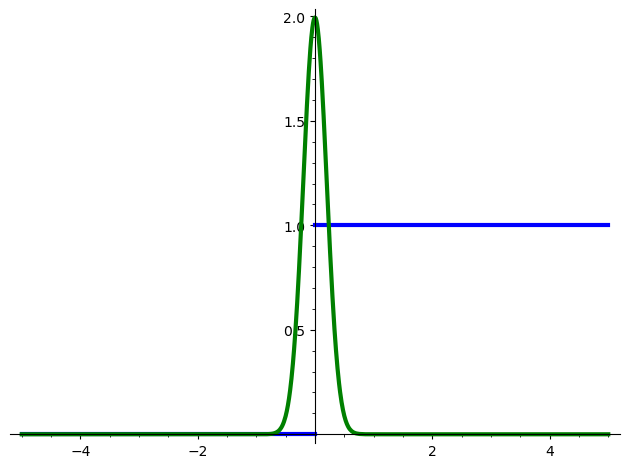
\includegraphics[width=0.5\textwidth]{graphics/heaviside}
\end{figure}

\begin{example}
The \dfn{Heaviside step function}\footnote{Named after Oliver Heaviside (1850--1925), an engineer who introduced an early version of the ``distributional calculus'' used to solve differential equations. Mathematicians did not consider the distributional calculus rigorous until the 1950s, however.}
\[H(x) = \begin{cases}
0, & x \leq 0\\
1, & x > 0
\end{cases}\]
is a useful example of a left-continuous function which is not continuous.
Clearly the derivative $H'(x)$ exists if $x \neq 0$, and in that case $H'(x) = 0$.
We want to say that $H'(0) = \infty$ in some suitable sense, and in fact that for any $\varepsilon > 0$,
\[\int_{-\infty}^{\infty} H'(x)~dx = \int_{-\varepsilon}^{\varepsilon} H'(x)~dx = 1.\]
Of course we can't do that, because the limit that would define $H'(0)$ does not exist.
See Figure \ref{Heaviside figure}.
\end{example}

\begin{definition}
Let $f: \RR \to \RR$ be a nondecreasing, left-continuous function.
Define
\[\mu_{f}([a, b)) = f(b) - f(a).\]
We call $\mu_{f}$ the \dfn{Stieltjes premeasure} of $f$.
\end{definition}

\begin{subsec}
A nondecreasing function can only be discontinuous on a countable set (Exercise~\ref{nondecreasing exercise}).
Thus we can turn a nondecreasing function $f$ into a left-continuous function $g$ by declaring that if $f$ is continuous at $x$ then $g(x) = f(x)$, and otherwise setting
\[g(x) = \lim_{\varepsilon \to 0} f(x - \varepsilon).\]
Henceforth we will talk about Stieltjes premeasures of any nondecreasing function, knowing that we may have to redefine them on a countable set in order that the definition make sense.
\end{subsec}

\begin{example}
If $f(x) = x$, then the Stieltjes premeasure of an interval $[a, b)$ under $f$ is just its length $b - a$.
This premeasure is known as the \dfn{Lebesgue premeasure}.
It will be by far the most important premeasure that we study.
If the following theory ever seems too abstract, try it out on the Lebesgue premeasure!
\end{example}

\begin{example}
The Stieltjes premeasure of a differentiable function $f$ can be thought of as ``weighted length''; $\mu_{f}([a, b)) > b - a$ provided that $f' > 1$ on $b - a$, and $\mu_{f}([a, b)) < b - a$ if $f' < 1$.
This is just an expression of the fundamental theorem of calculus: if $f$ is differentiable then
\[\mu_{f}([a, b)) = f(b) - f(a) = \int_{a}^{b} f'(x)~dx.\]
Since $f$ is nondecreasing, $f' \geq 0$.
This is our first clue that there is some connection between integration and measure theory.
\end{example}

\begin{example}
The Stieltjes premeasure of the Heaviside function $H$ will allow us to make some sense of our previous waffling about its derivative.
If $0 \notin [a, b)$ then $\mu_{H}([a, b)) = 0$.
Otherwise, $a \leq 0 < b$ and $H(b) = 1$, $H(a) = 0$; thus $\mu_{H}([a, b)) = 1$.
If one instead considers a finite set $X = \{x_{1}, \dots, x_{n}\}$ and
\[f(x) = \sum_{j=1}^{n} H(x - x_{j}),\]
then $\mu_{f}([a, b))$ is the cardinality of $X \cap [a, b)$.
\end{example}

\begin{theorem}
Every Stieltjes premeasure is $\sigma$-additive.
In particular, Lebesgue premeasure is $\sigma$-additive.
\end{theorem}
\begin{proof}
Let $\mu_{f}$ be a Stieltjes premeasure.
Let $E_{n} = [a_{n}, b_{n})$, assume that the $E_{n}$ are disjoint, and let $E = \bigcup_{n} E_{n}$.
Suppose that $E = [a, b)$. We must show
\begin{equation}\label{SPM sum}
f(b) - f(a) = \sum_{n=1}^{\infty} f(b_{n}) - f(a_{n}).
\end{equation}
To do so, we first note that since $f$ is nondecreasing, the quantities $\mu_{f}([a_{n}, b_{n}))$ are positive, so the sum in (\ref{SPM sum}) converges absolutely.
Thus we may rearrange the order of the summands without affecting the value of the sum, so we can assume that $a_{n} \leq a_{n+1}$ for every $n$, by reordering the intervals $E_{n}$.
Since the intervals are disjoint it follows that $b_{n} \leq a_{n+1}$.

We now prove
\[\mu_{f}(E) \geq \sum_{n=1}^{\infty} \mu_{f}(E_{n}).\]
To do this, we fix an $N$ and show that
\begin{equation}\label{SPM sum bound 1}
f(b) - f(a) \geq \sum_{n=1}^{N} f(b_{n}) - f(a_{n}).
\end{equation}
Now $b \geq b_{n}$ and $a \leq a_{n}$, so $f(b) - f(a) \geq f(b_{N}) - f(a_{1})$, but
\[\sum_{n=1}^{N} f(b_{n}) - f(a_{n}) = f(b_{N}) - f(a_{1}) + \sum_{n=1}^{N-1} f(b_{n}) - f(a_{n+1}).\]
But $b_{n} \leq a_{n+1}$ so $f(b_{n}) \leq f(a_{n+1})$, so
\[\sum_{n=1}^{N-1} f(b_{n}) - f(a_{n+1}) \leq 0.\]
Therefore
\[\sum_{n=1}^{N} f(b_{n}) - f(a_{n}) \leq f(b_{N}) - f(a_{1}) \leq f(b) - f(a).\]
This proves (\ref{SPM sum bound 1}).

Conversely, we must show that
\[\mu_{f}(E) \leq \sum_{n=1}^{\infty} \mu_{f}(E_{n}).\]
It suffices to show that for every $\varepsilon > 0$,
\begin{equation}\label{SPM sum bound 2}
f(b) - f(a) \leq \varepsilon + \sum_{n=1}^{\infty} f(b_{n}) - f(a_{n}).
\end{equation}
Now choose $b' < b$ such that $f(b') \geq f(b) - \varepsilon/2$ and for each $n$ choose $a_{n}' < a_{n}$ such that $f(a_{n}') \geq f(a_{n}) - \varepsilon/2^{n+1}$.
Such $a_{n}'$ and $b'$ exist because $f$ is left-continuous.
Now
\[[a_{n}', b'] \subseteq [a, b) = \bigcup_{n=1}^{\infty} [a_{n}, b_{n}) \subseteq \bigcup_{n=1}^{\infty} (a_{n}', b_{n}).\]
Therefore the $(a_{n}', b_{n})$ are an open cover of $[a_{n}', b]$, so by the Heine-Borel theorem there is an $N$ such that
\[[a_{n}', b'] \subseteq \bigcup_{n=1}^{N} (a_{n}', b_{n}).\]
If any interval is superfluous, we now discard it.
Then the way we ordered the intervals, $a_{n+1}' \leq b_{n}$.
TODO:\@ Draw a picture.
Moreover, $a_{1}' \leq a$ and $b' \leq b_{N}$. Then
\begin{align*}
f(b) - f(a) &\leq f(b') - f(a) + \frac{\varepsilon}{2}\\
& \leq f(b_{N}) - f(a_{1}') + \frac{\varepsilon}{2}\\
& \leq f(b_{N}) - f(a_{1}') + \frac{\varepsilon}{2} + \sum_{n=1}^{N-1} f(b_{n}) - f(a_{n+1}')\\
& \leq \frac{\varepsilon}{2} + \sum_{n=1}^{N} f(b_{n}) - f(a_{n}')\\
& \leq \frac{\varepsilon}{2} + \sum_{n=1}^{N} f(b_{n}) - f(a_{n}) + \frac{\varepsilon}{2^{n+1}}\\
& \leq \varepsilon + \sum_{n=1}^{N} f(b_{n}) - f(a_{n})
\end{align*}
where we used Zeno's paradox
\begin{equation}\label{zeno}
\sum_{n=1}^{\infty} \frac{1}{2^{n}} = 1
\end{equation}
to sum the geometric series of $\varepsilon$'s.
But this estimate is exactly (\ref{SPM sum bound 2}).
\end{proof}

\begin{exercise}\label{nondecreasing exercise}
Show that a nondecreasing function on $\RR$ can only be discontinuous on a countable set.
\end{exercise}

\begin{exercise}
Let $\Sigma$ be a $\sigma$-algebra, and let $\mu: \Sigma \to B$ be a function such that whenever $A_{1} \subseteq A_{2} \subseteq A_{3} \subseteq \cdots$,
\[\lim_{n \to \infty} \mu(A_{n}) = \mu\left(\bigcup_{n=1}^{\infty} A_{n}\right).\]
Show that if $\mu$ is \dfn{additive} (that is, if $A \cap B = \emptyset$, then $\mu(A \cup B) = \mu(A) + \mu(B)$), then $\mu$ is $\sigma$-additive.
\end{exercise}

\begin{exercise}
Let $\mathcal F$ be the vector space of left-continuous, nondecreasing functions and $\mathcal M$ the vector space of Stieltjes premeasures.
Show that the map $f \mapsto \mu_{f}$ which assigns a function to its Stieltjes premeasure is a linear map $\mathcal F \to \mathcal M$.
\end{exercise}

\section{Premeasures and outer measures}
Encouraged by the previous section, we now define premeasures in general.
Our goal is to define a $\sigma$-additive function that can be extended to a measure in a unique way; thus, to define a measure, it will suffice to define a premeasure.

\begin{definition}
A nonempty set $P$ of subsets of a set $X$ is said to be a \dfn{semiring}\footnote{The terminology is inspired by Exercise \ref{sigma algebras are rings}.} in $X$ if
\begin{enumerate}
\item For every $E, F \in P$, $E \cap F \in P$\footnote{A nonempty set of subsets of $X$ satisfying just this first condition is sometimes called a \dfn{$\pi$-system}, especially in probability theory.},
\item There are countably many sets $E_{1}, E_{2}, \dots \in P$ such that $\bigcup_{n} E_{n} = X$, and
\item For every $E, F \in P$, there are $G_{1}, \dots, G_{m}$ disjoint such that
\[E \setminus F = \bigcup_{n=1}^{m} G_{n}.\]
\end{enumerate}
A $\sigma$-additive function $P \to [0, \infty]$ which is not identically $\infty$ is called a \dfn{premeasure}.
\end{definition}

\begin{example}
The set of all half-open intervals $[a, b)$ is a semiring, so a Stieltjes premeasure is a premeasure.
\end{example}

\begin{lemma}\label{semiring prop 1}
Let $P$ be a semiring and $\mu$ a premeasure on $P$. Then:
\begin{enumerate}
\item If $E_{1}, \dots, E_{m} \in P$ then there are disjoint $F_{1}, \dots, F_{n} \in P$ such that
\[((((E_{1} \setminus E_{2}) \setminus E_{3}) \setminus \cdots) \setminus E_{m}) = \bigcup_{i=1}^{n} F_{i}.\]
\item $\mu(\emptyset) = 0$.
\end{enumerate}
\end{lemma}
\begin{proof}
Exercise~\ref{semiring exercise}.
\end{proof}

\begin{lemma}\label{semiring prop 2}
Let $P$ be a semiring and $\mu$ a premeasure on $P$. Then:
\begin{enumerate}
\item If ${(E_{n})}_{n}$ is a sequence of disjoint sets in $P$ and $E \supseteq \bigcup_{n} E_{n}$, $E \in P$, then
\[\sum_{n=1}^{\infty} \mu(E_{n}) \leq \mu(E).\]
\item If $E \subseteq F$, $E, F \in P$, then $\mu(E) \leq \mu(F)$.
\end{enumerate}
\end{lemma}
\begin{proof}
We first prove the first claim. By Lemma~\ref{semiring prop 1}, there are $F_{i} \in P$ disjoint such that
\[((((E_{1} \setminus E_{2}) \setminus E_{3}) \setminus \cdots) \setminus E_{m}) = \bigcup_{i=1}^{n} F_{i}.\]
In particular, $E$ is the disjoint union of the $E_{i}$ and $F_{i}$. Thus
\[\mu(E) = \sum_{i} \mu(E_{i}) + \sum_{j} \mu(F_{j}).\]
But $\mu$ is nonnegative so $\sum_{i} \mu(E_{i}) \geq 0$, thus the claim.

The second claim follows from the first in the case $n = 1$, $E_{1} = F$.
\end{proof}

\begin{subsec}
The power of Lemma~\ref{semiring prop 2} is that it does not assume that $\bigcup E_{n} \in P$.
\end{subsec}

\begin{subsec}
With these basic properties of premeasures set aside, we now discuss how to extend a premeasure to a measure.
First, we note that while premeasures are $\sigma$-additive, they also have another useful property, called $\sigma$-subadditivity.
\end{subsec}

\begin{definition}
Let $P$ be a set of sets. A function $\mu: P \to (-\infty, \infty]$ such that for every sequence of $E_{i} \in P$, if $E \in P$ and $E \subseteq \bigcup_{i} E_{i}$, then
\[\mu(E) \leq \sum_{i=1}^{\infty} \mu(E_{i}),\]
is said to be a \dfn{$\sigma$-subadditive function}.
\end{definition}

\begin{lemma}
Every premeasure is $\sigma$-subadditive.
\end{lemma}
\begin{proof}
Suppose that $E = \bigcup_{i} E_{i}$. By Lemma~\ref{semiring prop 1}, we can write
\[(((E_{i} \setminus E_{i-1}) \setminus E_{i-2}) \setminus \cdots \setminus E_{1}) = \bigcup_{j=1}^{k_{i}} F_{i}^{j}\]
where the $F_{i}^{j}$ are disjoint, hence
\[\mu(E) = \mu(E_{1}) + \sum_{i=2}^{\infty} \sum_{j=1}^{k_{i}} \mu(F_{i}^{j}).\]
But $\bigcup_{j} F_{i}^{j} \subseteq E_{i}$ so by Lemma~\ref{semiring prop 2},
\[\sum_{j=1}^{k_{i}} \mu(F_{i}^{j}) \leq \mu(E_{i}).\]
Thus
\[\mu(E) \leq \sum_{i=1}^{\infty} \mu(E_{i})\]
which was to be shown.
\end{proof}

\begin{subsec}
Because premeasures are $\sigma$-subadditive, it would be natural to extend them to a $\sigma$-subadditive function defined on a $\sigma$-algebra. Actually, since the set $2^{X}$ of all subsets of $X$ is already a $\sigma$-algebra (Exercise \ref{trivial sigma algebras}), we might as well take $2^{X}$ to be our $\sigma$-algebra.
\end{subsec}

\begin{definition}
An \dfn{outer measure} on $X$ is a $\sigma$-subadditive function $\omega: 2^{X} \to [0, \infty]$ such that $\omega(\emptyset) = 0$.
\end{definition}

\begin{subsec}
It follows from the definition that an outer measure $\omega$ is monotone; that is, if $E \subseteq F$, $E,F \in P$, then $\omega(E) \leq \omega(F)$.
\end{subsec}

\begin{subsec}
Let $P$ be a semiring in $X$ and $\mu$ be a premeasure on $P$. Now that we have made up our minds to extend $\mu$ to an outer measure $\mu^{*}$ on $X$, how should we do so?
As usual we turn to the example of the Lebesgue premeasure, so that
$$\mu([a, b)) = b - a$$
is the length of the half-open intervals $[a, b)$.

Imagine the half-open intervals to be like rulers.
If $E \subseteq \RR$ is a ``well-behaved" set, we expect that we can approximate the length of $E$ by covering $E$ with countably many rulers $[a_{n}, b_{n})$ and summing up the lengths of the rulers.
This will overestimate the length of $E$, both because the rulers may overlap and because $E \subseteq \bigcup_{n} [a_{n}, b_{n})$ but not conversely. See Figure \ref{rulers}.
But that's okay: maybe taking the limit as the rulers overestimate the length of $E$ less and less will get us the correct value of the length of $E$, which we denote $\mu^{*}(E)$.
We make this waffling more precise in the following definition.
\end{subsec}

\begin{figure}
\label{rulers}
\caption{We want to estimate the total length of the blue set $E$ by adding up the lengths of the rulers. The left side of the $n$th ruler is $a_{n}$ and the right side is $b_{n}$, so the length of the $n$th ruler is $b_{n} - a_{n}$. The rulers overlap and cover some points not in $E$, so the estimate $\sum_{n} b_{n} - a_{n}$ is slightly larger than the length of $E$.}
\centering 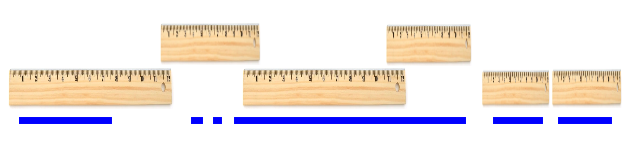
\includegraphics[width=0.75\textwidth]{graphics/rulers}
\end{figure}

\begin{definition}
Let $P$ be a semiring in $X$ and $\mu$ be a premeasure on $P$. For every $A \subseteq X$, define
\begin{equation}
\label{ruler formula}
\mu^{*}(A) = \inf \sum_{n=1}^{\infty} \mu(E_{n})
\end{equation}
where the $\inf$ ranges over all sequences of sets ${(E_{n})}_{n}$, $E_{n} \in P$, such that $A \subseteq \bigcup_{n} E_{n}$.
We call $\mu^{*}$ the \dfn{outer measure generated by $\mu$}.
\end{definition}

\begin{theorem}\label{extending premeasure to outer measure}
Let $P$ be a semiring and $\mu$ be a premeasure on $P$. Then the outer measure $\mu^{*}$ generated by $\mu$ is an outer measure on $X$ and for every $E \in P$, $\mu^{*}(E) = \mu(E)$.
\end{theorem}
\begin{proof}
We first note carefully that the infimum in (\ref{ruler formula}) is not vacuous; that is, for every $A \subseteq X$ there exists a sequence of sets ${(E_{n})}_{n}$, $E_{n} \in P$, such that $A \subseteq \bigcup_{n} E_{n}$.
Indeed, since $P$ is a semiring we can take the $E_{n}$ so that $\bigcup_{n} E_{n} = X$.

Now we check $\mu^{*}(\emptyset) = 0$. In fact, taking $E_{n} = \emptyset$ for every $n$, we have $\mu^{*}(\emptyset) \leq \sum_{n} 0 = 0$.

We now must show $\mu^{*}(A) = \mu(A)$ when $A \in P$. Clearly $\mu^{*}(A) \leq \mu(A)$.
Since $\mu$ is $\sigma$-subadditive, for any $E_{i} \in P$ such that $A \subseteq \bigcup_{i} E_{i}$, $\mu(A) \leq \sum_{i} \mu(E_{i})$, thus $\mu(A) \leq \mu^{*}(A)$.

Finally we show that $\mu^{*}$ is $\sigma$-subadditive. Suppose that
$$A \subseteq \bigcup_{n} A_{n} \subseteq X.$$
We must show
\[\mu^{*}(A) \leq \sum_{n=1}^{\infty} \mu^{*}(A_{n}).\]
Obviously this is true if some $\mu^{*}(A_{n}) = \infty$, so suppose that for every $n$, $\mu^{*}(A_{n}) < \infty$ and let $\varepsilon > 0$.
By definition of $\mu^{*}$, there are $E_{i}^{j} \in P$ such that $A_{i} \subseteq \bigcup_{j} E_{i}^{j}$
and
\[\mu^{*}(A_{i}) \geq \sum_{j=1}^{\infty} \mu(E_{i}^{j}) - \frac{\varepsilon}{2^{i}}.\]
Thus $A \subseteq \bigcup_{i,j}E_{i}^{j}$ whence
\begin{align*}\mu^{*}(A) &\leq \sum_{i,j} \mu(E_{i}^{j}) \leq \sum_{i,j=1}^{\infty} \mu(E_{i}^{j}) \leq \sum_{i=1}^{\infty} \mu^{*}(A_{i}) + \frac{\varepsilon}{2_{i}}\\& \leq \varepsilon + \sum_{i=1}^{\infty} \mu^{*}(A_{i}).\end{align*}
This was to be shown.
\end{proof}

\begin{subsec}\footnote{The rest of this section is an optional historical note.}
There is a dual approach to the extension of premeasures, introduced by Lebesgue.
He considered not just outer measures but \dfn{inner measures} defined by the relation
\[\mu_{*}(E) = \sup \sum_{n=1}^{\infty} \mu(E_{n})\]
where the $\sup$ ranges over all sequences of $E_{n} \in P$ such that $\bigcup_{n} E_{n} \subseteq P$ and the $E_{n}$ are disjoint.
Then Lebesgue proposed to study the $\sigma$-algebra of all sets whose inner and outer measures agree.
Note the asymmetry: for inner measure we need to assume that the $E_{n}$ are disjoint, or else we could ``double-count'' elements of $E$.
This asymmetry is the origin of several pathologies that make inner measures difficult to work with, and now this approach is considered nothing more than a historical footnote.
\end{subsec}

\begin{example}
An example of an oddity of inner measure comes from trying to compute the inner measure of the set $X$ of irrational numbers in $[0, 1]$.
Let $P$ be the semiring of intervals with rational endpoints in $[0, 1]$ and let $\mu$ be the Stieltjes premeasure on $P$ defined by $\mu([a, b)) = b - a$.
Then $\mu^{*}(X) = 1$.

To see this, let $x \in [0, 1]$; we will compute $\mu^{*}(\{x\})$. Let ${[x]}_{n}$ be a rational number such that ${[x]}_{n} < x < {[x]}_{n} + 1/n$; thus $\{x\} \subset [{[x]}_{n}, {[x]}_{n} + 1/n)$ and so
\[\mu^{*}(\{x\}) \leq \mu({[x]}_{n}, {[x]}_{n} + 1/n) = \frac{1}{n}\]
whence $\mu^{*}(\{x\}) = 0$.

Let ${(x_{n})}_{n}$ be an enumeration of the countable set $\QQ \cap [0, 1]$; by $\sigma$-subadditity,
\[\mu^{*}(\QQ \cap [0, 1]) \leq \sum_{n=1}^{\infty} \mu^{*}(\{x_{n}\}) = 0\]
but $X \cup (\QQ \cap [0, 1]) = [0, 1]$, so
\[1 = \mu([0, 1]) \leq \mu^{*}(X) + \mu^{*}(\QQ \cap [0, 1]) = \mu^{*}(X) + 0.\]
Therefore $\mu^{*}(X) \geq 1$, but $X \subseteq [0, 1]$ so $\mu^{*}(X) \leq 1$.

But there are no intervals in $P$ which are contained in $X$; thus the only element of $P$ contained in $E$ is $\emptyset$, so
\[\mu_{*}(E) = \sup 0 = 0.\]
Thus this seemingly reasonable way of defining an inner measure fails to measure the set of irrational numbers.
\end{example}

\begin{exercise}\label{semiring exercise}
Prove Lemma~\ref{semiring prop 1}.
\end{exercise}


\section{The Carathéodory construction}
Carathéodory\footnote{Constantin Carathéodory (1873--1950), a Greco-German mathematician who started work as an engineer working on the Asyut dam in Egypt. In addition to his results in measure theory, Carathéodory made contributions to isoperimetric problems, complex analysis, and thermodynamics.} introduced a modern approach that we now consider which avoids the issues with inner measures.
The idea is that, while an outer measure may not be a measure, there is a canonically defined $\sigma$-algebra on which the outer measure will restrict to a measure.
The elements of that $\sigma$-algebra will be called measurable sets.

\begin{definition}
Let $\omega$ be an outer measure on $X$.
An \dfn{$\omega$-measurable set} is a set $A \subseteq X$ such that for every $E \subseteq X$,
\begin{equation}\label{clean division}
\omega(E) = \omega(E \cap A) + \omega(E \setminus A).
\end{equation}
We let $\mathcal M(\omega$ denote the set of all $\omega$-measurable sets.
In the event that (\ref{clean division}) holds, we say that $A$ \dfn{cleanly divides} $E$, or that $(A, E)$ satisfies the \dfn{Carathéodory condition}.
\end{definition}

\begin{subsec}
Since an outer measure $\omega$ is subadditive, one already has
\[\omega(E) \leq \omega(E \cap A) + \omega(E \setminus A)\]
and so one just has to prove the opposite inequality
\begin{equation}\label{Caratheodory inequality}
\omega(E \cap A) + \omega(E \setminus A) \leq \omega(E)
\end{equation}
to verify the Carathéodory condition (\ref{clean division}).
We observe that trivially, $X$ is $\omega$-measurable, since (\ref{clean division}) says $\omega(E) = \omega(E) + \omega(\emptyset) = \omega(E) + 0$.
This also motivates why we assumed $\omega(\emptyset) = 0$ in the definition of an outer measure.
\end{subsec}

\begin{definition}
Let $\omega$ be an outer measure on $X$.
We say that a set $Z \subseteq X$ is \dfn{$\omega$-null} if $\omega(Z) = 0$.
We let $\mathcal N(\omega)$ denote the set of all $\omega$-null sets.
\end{definition}

\begin{subsec}
Let $\omega$ be an outer measure. Then $\emptyset$ is $\omega$-null by definition.
If $Z$ is $\omega$-null and $A \subseteq Z$, then $0 \leq \omega(A) \leq \omega(Z) = 0$ so $A$ is $\omega$-null.
Every measure $\mu$ is a premeasure and so extends to an outer measure; thus we may talk about the $\mu$-null sets, which are exactly those sets $E \subseteq X$ such that there is $F \supseteq X$ with $\mu(F) = 0$.
\end{subsec}

\begin{lemma}
\label{null sets are measurable}
For every outer measure $\omega$, $\mathcal N(\omega)$ is closed under countable union and $\mathcal N(\omega) \subseteq \mathcal M(\omega)$.
Moreover, if $A$ is $\omega$-measurable and $Z$ is $\omega$-null, then $A \cup Z$ and $A \setminus Z$ are $\omega$-measurable.
\end{lemma}
\begin{proof}
Let $Z$ be $\omega$-null. Then for every $E$, $E \cap Z$ is $\omega$-null, so
\[\omega(E \cap Z) + \omega(E \setminus Z) = 0 + \omega(E \setminus Z) \leq \omega(E),\]
which verifies Carathéodory's inequality (\ref{Caratheodory inequality}).
Thus $Z$ is $\omega$-measurable, so $\mathcal N(\omega) \subseteq \mathcal M(\omega)$.
If $A$ cleanly divides $E$ then clearly so do $A \cup Z$ and $A \setminus Z$, so null sets have no effect on measurability.
Countable subadditivity implies that $\mathcal N(\omega)$ is a $\sigma$-algebra.
\end{proof}

\begin{subsec}
The philosophy of measure theory is that null sets don't matter much.
For example, once we define integration, we will show that if $Z$ is a $\mu$-null set and $f$ is any integrable function, we will always have
$$\int_Z f(x) ~d\mu(x) = 0.$$
Since they're harmless, we might as well the null sets throw them in to the class of all measurable sets; this motivates the following definition.
By Lemma \ref{null sets are measurable}, this definition is not at all a strong assumption.
\end{subsec}

\begin{definition}
Let $(X, \Sigma, \mu)$ be a measured space.
If for every measurable set $E \in \Sigma$ such that $\mu(E) = 0$, every subset of $E$ is $\Sigma$-measurable, we say that $(X, \Sigma, \mu)$ is a \dfn{complete measured space}, or that $\mu$ is a \dfn{complete measure}.
\end{definition}

\begin{theorem}[Carathéodory]
For every outer measure $\omega$ on $\mathcal H$, $\mathcal M(\omega)$ is a $\sigma$-algebra and the restriction $\mu = \omega|\mathcal M(\omega)$ is a measure.
Furthermore, $(X, \mathcal M(\omega), \mu)$ is a complete measured space.
\end{theorem}
\begin{proof}
We start by checking some closure properties of $\mathcal M(\omega)$.

\begin{lemma}\label{measurable complements lemma}
If $A_{1}, A_{2}$ are $\omega$-measurable sets, then so is $A_{1} \setminus A_{2}$.
\end{lemma}
\begin{proof}
Since $E$ is the disjoint union of the sets $E \cap (A_{1} \cap A_{2})$, $E \cap (A_{1} \setminus A_{2})$, $E \cap (A_{2} \setminus A_{1})$, and $E \cap (A_{1} \cup A_{2})$, this follows from the fact that $A_{1}$ and $A_{2}$ divide each of the above sets cleanly.
We leave the details as Exercise~\ref{measurable complements}.
\end{proof}

\begin{lemma}\label{finite addition lemma}
If $A_{1}, A_{2}$ are $\omega$-measurable sets, then so is $A_{1} \cup A_{2}$.
Moreover, if $A_{1}, A_{2}$ are disjoint and $E$ is any set, then
$$\omega(E \cap (A_{1} \cup A_{2})) = \omega(E \cap A_{1}) + \omega(E \cap A_{2}).$$
\end{lemma}
\begin{proof}
Let $A = A_{1} \cup A_{2}$. Taking complements,
$$A = X \setminus (X \setminus A) = (X \setminus A_{1}) \setminus A_{2}$$
which is measurable by Lemma \ref{measurable complements lemma}.
We leave the rest of the proof as Exercise \ref{finite addition exercise}.
\end{proof}

\begin{lemma}
\label{countable additivity lemma}
Let $E \subseteq X$ be any set and let $A = \bigcup_{n}$ be a countable disjoint union of $\omega$-measurable sets. Then
$$\omega(A \cap E) = \sum_n \omega(A_{n} \cap E).$$
\end{lemma}
\begin{proof}
By induction on $k$ and Lemma \ref{finite addition lemma}, $B_{k} = \bigcup_{n < k} A_{n}$ is $\omega$-measurable and
$$\omega(B_{k} \cap E) = \sum_{n<k} \omega(A_{n} \cap E).$$
Since $\omega$ is monotone and $B_{k} \subseteq A$,
$$\omega(A \cap E) \geq \mu^{*}(B_{k} \cap E).$$
Thus, by $\sigma$-subadditivity,
$$\omega(A \cap E) \geq \lim_{k \to \infty} \omega(B_{k} \cap E) = \sum_n \omega(A_{n} \cap E) \geq \omega(A \cap E).$$
Thus $\omega(A \cap E) \leq \sum_n \omega(A_{n} \cap E) \leq \omega(A \cap E)$, which is what we were meant to show.
\end{proof}

By Lemma \ref{countable additivity lemma} applied with $E = X$, $\mu = \omega|\mathcal M(\omega)$ is $\sigma$-additive.
If $\mu(E) = 0$ then every $F \subseteq E$ lies in the hereditary set $\mathcal N(\omega)$, so $F$ is measurable by Lemma \ref{null sets are measurable}.
Therefore, if $\mathcal M(\omega)$ is a $\sigma$-algebra, then $(X, \mathcal M(\omega), \mu)$ is a complete measured space.
By Lemma \ref{measurable complements lemma}, we just need to check that $\mathcal M(\omega)$ is closed under countable union.

Let $A = \bigcup_{n} A_{n}$ be a countable union of measurable sets.
Replacing $A_{n}$ with $A_{n} \setminus (A_{1} \cup \cdots \cup A_{n-1})$ and using closure under complements (Lemma \ref{measurable complements lemma}) it is no loss to assume that the $A_{n}$ are disjoint.
Then by Lemma \ref{finite addition lemma}, for every set $E \subseteq X$,
\begin{equation}
\label{showing momega is a sigma algebra}
\sum_{n} \omega(E \cap A_{n}) + \omega(E \setminus A) \leq \omega(E).
\end{equation}
We leave the details as Exercise \ref{showing momega is a sigma algebra exercise}.
But we also have $\omega(E) \leq \sum_{n} \omega(E \cap A_{n}) + \omega(E \setminus A)$ by $\sigma$-subadditivity.
Since $E$ was arbitrary, $A \in \mathcal M(\omega)$.
\end{proof}

\begin{subsec}
A priori, Carathéodory's theorem is not actually very useful.
We have not established any control on when Carathéodory's inequality (\ref{Caratheodory inequality}) is true, so we do not know which sets are $\omega$-measurable.
For all we know, it could always be the case that $\mathcal M(\omega)$ is the trivial $\sigma$-algebra $\mathcal M(\omega) = \{\emptyset, X\}$.

Fortunately, this turns out to not be the case.
If $\omega$ is an outer measure which is generated by a premeasure $\mu$ on a semiring $P$, then every subset of $P$ is measurable, as we now show.
(For example, if $P$ is the semiring of half-open intervals, then every Borel set will be $\omega$-measurable.)
Furthermore, if $\mu$ is ``not too big" in a sense that we will shortly make precise, then the measure obtained from Carathéodory's theorem is the unique extension of $\mu$ to a complete measured space.
Thus, to specify a measure, which in general is a horribly complicated object, we just need to give a premeasure defined on some semiring.
\end{subsec}

\begin{theorem}\label{Caratheodory 2}
Let $P$ a semiring in $X$ and let $\mu$ be a premeasure on $P$.
Then there is a $\sigma$-algebra $\Sigma$ which contains $P$ and an extension of $\mu$ to a complete measure on $\Sigma$.
\end{theorem}
\begin{proof}
Let $\omega$ be the outer measure generated by $\mu$ and let $\Sigma = \mathcal M(\omega)$,.
Then $(X, \Sigma, \omega|\Sigma)$ is a complete measured space, and by Theorem \ref{extending premeasure to outer measure}, $\omega|P = \mu$.

Suppose that $A \in P$ and $E \subseteq X$. We must verify Carathéodory's inequality (\ref{Caratheodory inequality}) in order to show $A \in \Sigma$.
If $\omega(E) = \infty$ then clearly (\ref{Caratheodory inequality}) holds.
Otherwise, suppose that $\omega(E) < \infty$ and $\varepsilon > 0$; we will show
\begin{equation}
\label{Caratheodory with epsilon}
\omega(E \cap A) + \omega(E \setminus A) \leq \omega(A) + \varepsilon.
\end{equation}

Since the infimum in (\ref{ruler formula}) is not vacuous (since $P$ is a semiring), the definition of $\omega$ implies that there exist countably many sets $F_{n} \in P$ such that $E \subseteq \bigcup_{n} F_{n}$ and
\begin{equation}
\label{Caratheodory overestimate}
\sum_{n} \mu_{0}(F_{n}) \leq \varepsilon + \omega(E).
\end{equation}
But $F_{n} = (A \cap F_{n}) \cup (F_{n} \setminus A)$, a disjoint union, so since $P$ is a semiring, there exist disjoint $G_{ij} \in P$ such that
$$F_{i} = (A \cap F_{i}) \cup \bigcup_{j=1}^{k_{i}} G_{ij}.$$
Then
$$\sum_{i} \mu(F_{i}) = \sum_{i} \mu(A \cap F_{i}) + \sum_{i} \sum_{j=1}^{k_{i}} \mu(G_{ij}).$$
Since $F_{i} \setminus A = \bigcup_{j \leq k_{i}} G_{ij}$ and $E \setminus A \subseteq \bigcup_{i} F_{i} \setminus A$,
$$E \setminus A \subseteq \bigcup_{i} \bigcup_{j=1}^{k_{i}} G_{ij}.$$
Combining this inequality with the inequality $A \cap E \subseteq \bigcup_{i} A \cap F_{i}$ and the inequality (\ref{Caratheodory overestimate}), we conclude
$$\omega(E \cap A) + \omega(E \setminus A) \leq \sum_{i=1}^\infty \omega(F_{i} \cap A) + \sum_{j=1}^{k_{i}} \omega(G_{ij}) = \sum_{i=1}^\infty \omega(F_{i}) \leq \omega(A) + \varepsilon$$
which implies (\ref{Caratheodory with epsilon}).
\end{proof}

\begin{subsec}
Now let us show that the complete measured space in Theorem \ref{Caratheodory 2} is unique, subject to the following assumption.
\end{subsec}

\begin{definition}
Let $\mu: \Sigma \to [0, \infty]$ be a measure, premeasure, or outer measure.
We say that $\mu$ is \dfn{$\sigma$-finite} if there are countably many $E_{n} \in \Sigma$ such that $\bigcup_{n} E_{n} = X$ and $\mu(E_{n}) < \infty$.
\end{definition}

\begin{subsec}
``Most" measures that one encounters in practice will be $\sigma$-finite, and pathological counterexamples can often be found by considering non-$\sigma$-finite measures.
As we shall see, non-$\sigma$-finite premeasures may not extend uniquely; much later on we will show, among other thing, that for non-$\sigma$-finite measures, the familiar formula
$$\int_X \int_Y f(x, y) ~d\mu(x) ~d\nu(y) = \int_Y \int_X f(x, y) ~d\nu(y) ~d\mu(x)$$
that one learns in calculus is false.

One can think of measure theory as a generalization of combinatorics, since the counting measure $\mu$ on a set $X$ satisfies $\mu(E) = \card E$ for every finite set $E \subseteq X$.
Thus $\sigma$-finite measures can be viewed as a generalization of countable sets, and the fact that non-$\sigma$-finite measures are pathological is analogous to the fact that in combinatorics, uncountable sets are complicated and need an additional theory of ``infinitary combinatorics".
\end{subsec}

\begin{theorem}\label{unique extensions}
Let $P$ a semiring in $X$ and let $\mu_{0}$ be a $\sigma$-finite premeasure on $P$.
Then there is a unique complete measured space $(X, \Sigma, \mu)$ such that $P \subseteq \Sigma$ and $\mu|P = \mu_{0}$.
Furthermore, $\mu$ is $\sigma$-finite and $\Sigma$ is the smallest $\sigma$-algebra containing $P$ and every $\mu$-null set.
\end{theorem}
\begin{proof}
By Theorem~\ref{Caratheodory 2}, $(X, \Sigma, \mu)$ exists.
Moreover, $\mu$ is still $\sigma$-finite, since if we have countably many sets $E_{n}$ for which $\mu_{0}(E_{n}) < \infty$ and $\bigcup_{n} E_{n} = X$, then the same holds with $\mu_{0}$ replaced with $\mu$.

We now show must uniqueness, so let $(X, \Gamma, \nu)$ be another complete measured space such that $P \subseteq \Gamma$ and $\nu|P = \mu_{0}$.

\end{proof}

\begin{definition}
Let $X$ be a topological space.
A \dfn{Borel measure} on $X$ is a measure $\Sigma \to [0, \infty]$ such that every Borel subset of $X$ is an element of $\Sigma$.
\end{definition}

\begin{theorem}
Every Stieltjes premeasure extends uniquely to a complete $\sigma$-finite Borel measure on $\RR$.
\end{theorem}
\begin{proof}
Let $\mu_{0}$ be the Stieltjes premeasure of an increasing right-continuous function $f$; then $\mu_{0}([n, n + 1)) = f(n + 1) - f(n) < \infty$, and the $[n, n + 1)$, $n \in \ZZ$, are a countable set of sets which cover $\RR$.
Therefore $\mu_{0}$ is $\sigma$-finite.
So, by Theorem~\ref{unique extensions}, $\mu_{0}$ extends uniquely to a complete $\sigma$-finite measure on a $\sigma$-algebra $\Sigma$ which contains every half-open interval.
But the half-open intervals generate the Borel $\sigma$-algebra of $\RR$ (Exercise \ref{generators of Borel}), so $\Sigma$ contains every Borel subset of $\RR$.
\end{proof}

\begin{definition}
A \dfn{Stieltjes measure} is the unique complete Borel measure that extends a Stieltjes premeasure.
\end{definition}

\begin{exercise}\label{measurable complements}
Complete the proof of Lemma~\ref{measurable complements lemma}.
\end{exercise}

\begin{exercise}\label{finite addition exercise}
Complete the proof of Lemma~\ref{finite addition lemma}.
\end{exercise}

\begin{exercise}\label{showing momega is a sigma algebra exercise}
Complete the proof of (\ref{showing momega is a sigma algebra}).
\end{exercise}

\begin{exercise}
Let $\mu$ be the Lebesgue premeasure, $\mu([a, b)) = b - a$, and let $Z \subseteq \RR$ be a countable set.
Show that $Z$ is $\mu^{*}$-null.
\end{exercise}

\begin{exercise}
Let $(X, \Sigma, \mu)$ be a measured space. Show that the following are equivalent:
\begin{enumerate}
\item $\mu$ is $\sigma$-finite.
\item There are countably many disjoint $E_{i} \in \Sigma$, $\mu(E_{i}) < \infty$, such that $\bigcup_{i} E_{i} = X$.
\item There are countably many $E_{i} \in \Sigma$, $\mu(E_{i}) < \infty$, such that $E_{i} \subseteq E_{i+1}$ and $\bigcup_{i} E_{i} = X$.
\end{enumerate}
These equivalences are highly useful and will be used throughout the text without explicit mention.
\end{exercise}

\begin{exercise}
Let $(X, \Sigma, \mu)$ be a measured space, and let $\mathcal N$ be the set of all $\mu$-null sets.
Let $\overline \Sigma$ be the $\sigma$-algebra generated by $\Sigma$ and $\mathcal N$.
Show that there is a unique extension $\overline \mu$ of $\mu$ to $(X, \overline \Sigma)$, and that $(X, \overline \Sigma, \overline \mu)$ is a complete measured space.
We call $(X, \overline \Sigma, \overline \mu)$ the \dfn{completion} of $(X, \Sigma, \mu)$.
\end{exercise}

\section{Lebesgue measure on $\RR$}
In this section we define the most important measure of all: Lebesgue measure on $\RR$.

\begin{definition}
The \dfn{Stieltjes measure} arising from a nondecreasing left-continuous function $f$ is the complete Borel measure $\mu_{f}$ obtained from the Stieltjes premeasure of $f$.
\end{definition}

\begin{lemma}
If $\mu_{f}$ is a Stieltjes measure then for every open interval $(\alpha, \beta)$ one has
\[\mu_{f}((\alpha, \beta)) = f(\beta) - \lim_{n \to \infty} f(\alpha + 1/n).\]
In particular, if $f$ is continuous then $\mu_{f}((\alpha, \beta)) = f(\beta) - f(\alpha)$.
\end{lemma}
\begin{proof}
By continuity of measure,
\[\mu_{f}((\alpha, \beta)) = \lim_{n \to \infty} \mu_{f}([\alpha + 1/n, \beta)) = \lim_{n \to \infty} f(\beta) - f(\alpha + 1/n)\]
which is what we wanted.
\end{proof}

\begin{subsec}
In particular, if $f(x) = x$, then $\mu_{f}((\alpha, \beta)) = \beta - \alpha$.
This fact will be used so often that we will frequently use it without reference.
\end{subsec}

\begin{definition}
The \dfn{Lebesgue measure} on $\RR$ is the Stieltjes measure arising from the Lebesgue premeasure; that is, the Lebesgue measure is $\mu_{f}$ where $f(x) = x$.
\end{definition}

\begin{subsec}
Let $\mu$ denote Lebesgue measure; then $\mu([\alpha, \beta)) = \beta - \alpha$ is the length of the interval $[\alpha, \beta)$.
Therefore $\mu$ is the natural generalization of ``length'' to as many subsets of $\RR$ as one reasonably can generalize it to.
Indeed, if $A$ is a Lebesgue measurable subset of $\RR$ (e.g.\ if $A$ is Borel) then
\begin{equation}\label{lebesgue measure formula}
\mu(A) = \inf \left\{\sum_{j=1}^{\infty} \beta_{i} - \alpha_{i}: A \subseteq \bigcup_{i=1}^{\infty} [\alpha_{i}, \beta_{i})\right\}.
\end{equation}
\end{subsec}

\begin{theorem}\label{translation invariance in R1}
Lebesgue measure $\mu$ is \dfn{translation-invariant} in the sense that if $A$ is a Lebesgue measurable set, and $A + x = \{a + x: a \in A\}$, then $\mu(A) = \mu(A + x)$.
Conversely, if $\nu$ is a translation-invariant complete Borel measure such that $\nu([0, 1)) = 1$, then $\mu = \nu$.
\end{theorem}
\begin{proof}
If $A = [\alpha, \beta)$ is an interval, then $\mu(A + x) = \beta + x - \alpha - x = \beta - \alpha = \mu(A)$.
If $A$ is an arbitrary measurable set, then by (\ref{lebesgue measure formula}),
\begin{align*}
\mu(A + x) &= \inf \left\{\sum_{j=1}^{\infty} \beta_{i} - \alpha_{i}: A + x\subseteq \bigcup_{i=1}^{\infty} [\alpha_{i}, \beta_{i})\right\} \\
&= \inf \left\{\sum_{j=1}^{\infty} \beta_{i} + x- \alpha_{i} - x: A \subseteq \bigcup_{i=1}^{\infty} [\alpha_{i}, \beta_{i})\right\}\\
&= \inf \left\{\sum_{j=1}^{\infty} \beta_{i} - \alpha_{i}: A \subseteq \bigcup_{i=1}^{\infty} [\alpha_{i}, \beta_{i})\right\}\\
&= \mu(A).
\end{align*}

Conversely, $\nu$ is $\sigma$-finite, since by translation invariance, the sets $[n, n + 1)$ all have $\nu$-measure $1$, there are countably many of them, and they cover $\RR$.
Now if $[\alpha, \beta)$ is an arbitrary interval, we can write
\[[\alpha, \beta) = \bigcup_{n\in\ZZ} [\alpha, \beta) \cap [n, n + 1)\]
and use countable additivity to see that
\[\nu([\alpha, \beta)) = \sum_{n\in\ZZ} \nu([\alpha, \beta) \cap [n, n + 1)).\]
So it suffices to show that $\nu([\alpha, \beta)) = \mu([\alpha, \beta))$ whenever $[\alpha, \beta) \subseteq [n, n + 1)$ for some $n$, in order that this also be true for any interval $[\alpha, \beta)$.
Then by translation invariance, it suffices to check this when $\alpha = 0$, in which case $\beta \in (0, 1)$.

Suppose first that $\beta$ is rational, say $\beta = p/q$. Then by translation invariance and countable additivity,
\[\nu([\alpha, \beta)) = \nu([0, p/q)) = \sum_{j=0}^{p-1} \nu([j, (j+1)/q)) = p\nu([0, 1/q)).\]
But
\[1 = \nu([0, 1)) = \sum_{j=0}^{q-1} \nu([j, (j+1)/q)) = q\nu([0, 1/q))\]
which implies that $\nu([0, 1/q)) = 1/q$ and hence $\nu([0, p/q)) = p/q$; therefore $\nu([\alpha, \beta)) = \beta - \alpha$ whenever $\beta - \alpha$ is rational.
If $\beta - \alpha$ is irrational, choose $\beta_{n} > \beta_{n+1} > \cdots > \beta$ so that $\beta_{n} \to \beta$ and $\beta_{n} - \alpha$ is rational for all $n$; then $\nu([\alpha, \beta_{n})) = \beta_{n} - \alpha$, so continuity of measure implies that $\nu([\alpha, \beta)) = \beta - \alpha$.

Since $\mu([\alpha, \beta)) = \nu([\alpha, \beta))$ for all $\alpha < \beta$, uniqueness of the Carathéodory construction for $\sigma$-finite measures implies that $\mu = \nu$.
\end{proof}

\begin{subsec}
The above argument is an example of a ``bootstrapping'' strategy that is common in measure theory.
Once one has established a simple case (here $\nu([0, 1)) = 1$), it is often possible to propagate that case to a slightly more complicated case ($\nu([0, 1/q)) = 1/q$, say), and then repeat this process until all sets of interest have been considered.
If you find yourself stuck on an exercise, it is worth trying to prove the claim in the simplest possible case and then iteratively improving the cases your proof works for until all cases are hit.
\end{subsec}

\begin{subsec}
Theorem~\ref{translation invariance in R1} shows that we could have defined Lebesgue measure axiomatically. We would have had to demanded that:
\begin{enumerate}
\item Countable additivity: Lebesgue measure be a measure.
\item Borel: Every open interval be Lebesgue measurable.
\item Completeness: Every subset of a Lebesgue null set be null.
\item Translation-invariance: A translate of a Lebesgue measurable set have the same Lebesgue measurable.
\item Calibration: The interval $[0, 1)$ have Lebesgue measure $1$.
\end{enumerate}
Certainly all of these conditions seem quite tame; then the Carathéodory construction would have proven existence and uniqueness.
However, it is convenient to pass through the notion of a Stieltjes measure along the way, as more general Stieltjes measures are quite useful in their own right.
\end{subsec}

\begin{subsec}
One may wonder if \emph{every} subset of $\RR$ is Lebesgue measurable.
Under certain reasonable set-theoretic hypotheses, this is false; we discuss a counterexample, Vitali's set, in Theorem~\ref{Vitali's set}.
But the next-best thing is true, as any set that an analyst, algebraist, topologist, or applied mathematician will ever have to work with will turn out to be measurable. We discuss this in Example~\ref{all functions are measurable}.
This is closely related to a theorem of Solovay~\cite{Solovay1970} which shows that in a certain sense, those set-theoretic hypotheses \emph{cannot} be avoided in the construction of a nonmeasurable set: a slightly different logical setup would imply that every subset of $\RR$ is measurable.
\end{subsec}

\begin{subsec}
Lebesgue measure is remarkably well-behaved, along with satisfying the five axioms above.
To see an example of another good property of Lebesgue measure, we need a new definition.
If the reader is uncomfortable with the abstract definition of a locally compact Hausdorff space, they may take $X = \RR$ in the following definition without losing any insight.
\end{subsec}

\begin{definition}\label{dfn of radon measure}
Let $X$ be a locally compact Hausdorff space.
Suppose that $\mu$ is a Borel measure on $X$ such that:
\begin{enumerate}
\item \dfn{Outer regularity}: For every Borel set $W$,
\[\mu(W) = \inf_{U} \mu(U)\]
where the infimum is taken over all open sets $U \supseteq W$.
\item \dfn{Inner regularity for open sets}: For every open set $U$,
\[\mu(U) = \sup_{K} \mu(K)\]
where the supremum is taken over all compact sets $K \subseteq U$.
\item \dfn{Local finiteness}: For every compact set $K$, $\mu(K) < \infty$.
\end{enumerate}
Then we say that $\mu$ is a \dfn{Radon measure}.
\end{definition}

\begin{theorem}\label{lebesgue is radon}
Every Stieltjes measure on $\RR$ is Radon.
In particular, Lebesgue measure is Radon.
\end{theorem}
\begin{proof}
Let $f$ be a nondecreasing left-continuous function.
If $K$ is compact then $K$ is bounded, so $K$ is contained in an interval $[\alpha, \beta)$ so $\mu_{f}(K) \leq f(\beta) - f(\alpha)$.
Therefore $\mu_{f}$ is locally finite.

For inner regularity, note that every open set $U$ can be written as a disjoint union of countably many open intervals, so it suffices to check when $U$ is the interval $(\alpha, \beta)$.
Now if $K \subset (\alpha, \beta)$ is compact then there is an $n$ such that $K \subseteq [\alpha + 1/n, \beta)$, so $\mu_{f}(K) \leq f(\beta) - f(\alpha + 1/n)$.
On the other hand,
\[\lim_{n \to \infty} \mu_{f}([\alpha + 1/n, \beta)) = f(\beta) - \lim_{n \to \infty} f(\alpha + 1/n) = \mu_{f}((\alpha, \beta)).\]
Therefore $\mu_{f}$ is inner regular.

For outer regularity, let $W$ be a Borel set (actually, any Stieltjes measurable set); then
\[\mu(W) = \inf_{(\alpha_{n}), (\beta_{n})} \sum_{n} f(\beta_{n}) - f(\alpha_{n})\]
where the $\inf$ ranges over all sequences of $\alpha_{n}$ and $\beta_{n}$ such that $W \subseteq \bigcup_{n} [\alpha_{n}, \beta_{n})$.
Fix any such sequences.
Now $E_{m}^{n} = (\alpha_{n} - m^{-1}2^{-n}, \beta_{n})$ is an open cover of $W$ for any $m$, so
\[\mu(W) \leq \sum_{n} f(\beta_{n}) - f(\alpha_{n}) < \frac{1}{m} + \sum_{n} f(\beta_{n}) - f(\alpha_{n}) = \sum_{n} f(\beta_{n}) - f(\alpha_{n}) + m^{-1}2^{-n}.\]
Taking $m \to \infty$ and minimizing $\sum_{n} f(\beta_{n}) - f(\alpha_{n})$ by varying the $\alpha_{n}$ and $\beta_{n}$ we collapse the above inequalities into $\inf$s.
\end{proof}

\begin{subsec}
The proof of Theorem~\ref{lebesgue is radon} shows that Stieltjes measures are not just outer regular for Borel sets, but outer regular for any Stieltjes measurable set whatsoever.
However, this fact is rarely useful; as discussed below, we are mainly interested in equivalence classes of sets modulo null sets, and every Lebesgue measurable set is equivalent under that equivalence relation to a Borel set.
\end{subsec}

\begin{subsec}
After this chapter, we will mainly be interested in not measurable sets, but rather equivalence classes of measurable sets under the equivalence relation ``symmetric difference is a null set''.
That is, we think of two measurable sets $A,B$ as the same if the symmetric difference $A \Delta B = (A \setminus B) \cup (B \setminus A)$ is null.
For example, every countable set is the same as the empty set.
One can give a different construction of the Lebesgue measure if one is \emph{only} interested in equivalence classes of measurable sets, rather than measurable sets themselves; see Exercises~\ref{physical lebesgue measure 1} through~\ref{physical lebesgue measure 3}.
\end{subsec}

\begin{figure}
\label{Cantor set figure}
\caption{The sets $C_{0}, \dots, C_{4}$ used in the construction of the Cantor set.}
\centering 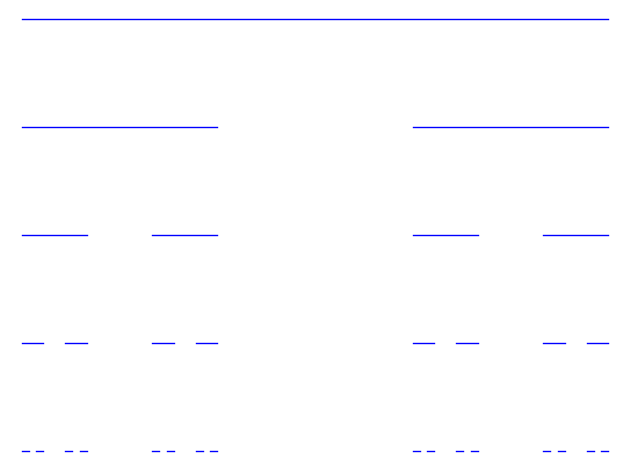
\includegraphics[width=0.5\textwidth]{graphics/CantorSet}
\end{figure}

\begin{subsec}
Let us now construct a useful example of an uncountable, null compact set, known as the \dfn{standard Cantor set}.
This set will frequently be useful as an example, and will be treated at length in the exercises.

Let $C_{0} = [0, 1]$, and given $C_{n}$ a finite union of closed intervals, let $C_{n+1}$ consist of $C_{n}$ with the open middle-thirds of each interval in $C_{n}$ removed.
See Figure \ref{Cantor set figure}.
Let $C$, the standard Cantor set, be defined by $C = \bigcap_{n} C_{n}$.
\end{subsec}

\begin{subsec}
It is often convenient to view the Cantor set in the following way. Let $2$ be a shorthand for the set $\{0, 1\}$.
Let $2^{\omega}$ denote the space of sequences in $2$, thus $2^{\omega}$ is the set of all functions $\NN \to \{0, 1\}$.

For each $x \in 2^{\omega}$, we obtain a point $f(x) \in C$ in the following way.
Assume that $D_{n-1}$ is one of the closed intervals obtained in stage $n-1$ of the Cantor set construction, thus $D_{n-1}$ is an interval in $C_{n-1}$.
If $x_{n} = 0$, let $D_{n}$ be the left closed interval in $D_{n-1}$, and otherwise let $D_{n}$ be the right closed interval.
Then $D_{n} \subseteq D_{n-1} \cap C_{n}$.
The intersection of closed nonempty intervals is a closed nonempty interval, so we obtain such an interval $D \subseteq C$.
But a consequence of Exercise~\ref{Cantor set props} is that the Cantor set contains no nontrivial intervals, so $D$ consists of a single point $f(x)$.

The map $f$ is injective since if $f(x) = f(y)$ then, at the $n$th stage of the Cantor set construction, both $x$ and $y$ agreed on which subinterval to pass to, thus $x = y$.
It is surjective since every point $p \in C$ must be in some interval $D_{n}$ at stage $n$, and if $D_{n}$ is the left interval of $D_{n-1}$ then we can set $x = 0$, and otherwise set $x = 1$; then $f(x) = p$.
One can similarly interpret the Cantor set as the set of all paths through the full infinite binary tree.
This perspective can be highly useful in some exercises and in applications.
For more on Cantor sets, see Pugh~\cite[Chapter 2]{pugh2013real}.
\end{subsec}

\begin{exercise}
Let $x \in \RR$ and let $f$ be a nondecreasing, left-continuous function. Show that
\[\mu_{f}(\{x\}) = \lim_{\varepsilon \to 0} f(x+\varepsilon) - f(x).\]
Conclude that if $f$ is continuous, then $\mu_{f}$ makes all countable sets null.
\end{exercise}

\begin{exercise}
Let $f$ be a nondecreasing, left-continuous function. Show that there is a nonempty open set $U$ such that $\mu_{f}(U) = 0$ iff $f$ is not strictly increasing (i.e.\ there are $x < y$ with $f(x) = f(y)$).
\end{exercise}

\begin{exercise}\label{Dirac measure}
Let $x \in \RR$. The \dfn{Dirac measure} at $x$, denoted $\delta_{x}$, is the Stieltjes measure arising from the function
\[y \mapsto \begin{cases}
0, &y \leq x\\
1, &y > x.
\end{cases}\]
A set is \dfn{Dirac measurable} at $x$ if it is measurable with respect to $\delta_{x}$.
Show that every subset of $\RR$ is Dirac measurable at $x$, and compute its Dirac measure.
\end{exercise}

\begin{exercise}\label{Cantor set props}
Show that the standard Cantor set is compact and Lebesgue null, has the same cardinality as $\RR$, and contains no interval except for points and the empty set.
\end{exercise}

\begin{exercise}
Let $\mu$ denote Lebesgue measure on $\RR$.
Show that there is a Borel probability measure $\nu$ on $\RR$, such that for every countable set $A$, $\nu(A) = 0$, and if $\mu(A) > 0$, then $\nu(A) = 0$.
(Hint: Define $\nu$ in such a way that, if $C$ denotes the standard Cantor set, then $\nu(C) = 1$, and use Exercise~\ref{Cantor set props}.)
\end{exercise}

\begin{exercise}
Show that the set of Lebesgue measurable subsets of $\RR$ has cardinality equal to that of the power set $2^{\RR}$ of $\RR$. Conclude that there exists a Lebesgue measurable set which is not Borel.
(Hint: Exercise~\ref{Cantor set props}.)
\end{exercise}

\begin{exercise}\label{fat cat}
Show that for every $\alpha \in [0, 1)$ there exists a Cantoresque subset $C_{\alpha}$ of $[0, 1]$ whose Lebesgue measure is $\alpha$.
In particular, $C_{\alpha}$ should be compact and contain no open subset of $\RR$.
This is known as a \dfn{fat Cantor set}.
Show that there does not exist a fat Cantor set of measure $1$ in $[0, 1]$.
\end{exercise}

\begin{exercise}
Show that every locally finite Borel measure on $\RR$ is Stieltjes (and hence Radon).
\end{exercise}

\begin{exercise}\label{physical lebesgue measure 1}
In this exercise and the following we give a different construction of Lebesgue measure, other than the axiomatic definition or the construction using Stieltjes measures.

Let $\Sigma_{0}$ be the set of all intervals (open, closed, or half-open) with rational endpoints.
Given $I \in \Sigma_{0}$, define $\nu(I)$ to be the length of $I$.
If $I, J \in \Sigma_{0}$, then $I \setminus J \in \Sigma_{0}$, so we can define
\[d_{0}(I, J) = \nu(I \setminus J) + \nu(J \setminus I).\]
Show that $d_{0}$ is a semimetric, so the completion $(\Sigma, d)$ of $(\Sigma_{0}, d_{0})$ is a complete metric space, and $\nu$ is a continuous function on $\Sigma$.

Show that the ``union'' of countably many elements of $\Sigma$ is well-defined, as is the ``intersection'' of countably many elements and ``complement'' of one element.
That is, show that these operations drop to equivalence classes of elements of $\Sigma_{0}$ under the equivalence relation ``distance is $0$'', and then extend uniquely to $\Sigma$.
So $\Sigma$ can be thought of as an ``abstract $\sigma$-algebra'' in some sense, even though its elements are not sets, but something more abstract.
\end{exercise}

\begin{exercise}\label{physical lebesgue measure 2}
Let all definitions be as Exercise~\ref{physical lebesgue measure 1}.
Given $J \in \Sigma_{0}$, define $[J]$ to be the equivalence class of $J$ in $\Sigma$.
Then, given $I \in \Sigma$, let
\[\nu(I) = d(I, [\emptyset]).\]
Show that $\nu$ is ``$\sigma$-additive'' in the sense that whenever ${(E_{n})}_{n}$ is a sequence in $\Sigma$ with $E_{n} \cap E_{m} = [\emptyset]$ whenever $n \neq m$, then
\[\nu\left(\bigcup_{n} E_{n}\right) = \sum_{n} \nu(E_{n}).\]
So we can think of $\nu$ as an ``abstract measure'' on the abstract $\sigma$-algebra $\Sigma$.
We call $\nu$ the \dfn{physical Lebesgue measure}.
\end{exercise}

\begin{exercise}\label{physical lebesgue measure 3}
Let $\mu$ be Lebesgue measure and $\nu$ physical Lebesgue measure as in Exercise~\ref{physical lebesgue measure 2}, defined on the abstract $\sigma$-algebra $\Sigma$.
Let $\Gamma$ be the $\sigma$-algebra of Lebesgue measurable subsets of $\RR$. Show that there is a surjective map $\pi: \Gamma \to \Sigma$ such that:
\begin{enumerate}
\item For every rational interval $I$, $\pi(I)$ is the equivalence class of $I$ in $\Sigma$.
\item For every sequence ${(E_{n})}_{n}$ in $\Gamma$, $\pi(\bigcup_{n} E_{n}) = \bigcup_{n} \pi(E_{n})$, and similarly for intersection and complement.
\item For every $E \in \Gamma$, $\mu(E) = \nu(\pi(E))$.
\end{enumerate}
So we can think of $\pi(E)$ as the equivalence class of $E$ under the equivalence relation ``symmetric difference is null'', and $\nu$ correctly computes the Lebesgue measurable of a set.
\end{exercise}

\section{Vector-valued measures}
Recall that by definition, a measure $\mu$ is a $\sigma$-additive function $\mu: \Sigma \to (-\infty, \infty]$, where $\Sigma$ is a $\sigma$-algebra.
However, the definition of $\sigma$-additive function makes sense even if $(-\infty, \infty]$ is replaced by a more general codomain, and we will have use for this when we integrate functions in more general codomains than the real numbers.

\begin{subsec}
Let $B$ be a Banach space, as discussed in Appendix~\ref{Banach space appendix}.
If the reader is unfamiliar with Banach spaces, they can take $B = \CC^{d}$ and not lose any insight.
If $(x_{n})$ is a sequence in $B$, then (\ref{banach space series}) is the definition of the infinite sum $\sum_{n} x_{n}$.
\end{subsec}

\begin{definition}
Let $\Sigma$ be a $\sigma$-ring and $B$ a Banach space.
A \dfn{vector-valued measure} on $\Sigma$, or simply a \dfn{measure}, is a function $\mu: \Sigma \to B$ such that whenever $(E_{n})$ are countably many disjoint sets in $\Sigma$,
\[\mu\left(\bigcup_{n} E_{n}\right) = \sum_{n} \mu(E_{n}).\]
\end{definition}

\begin{example}
The most important examples of vector-valued measures will be of the following form.
Let $\nu$ be a positive measure on a measurable space $X$, and let $f: X \to B$ be an ``integrable function''.
We will get back to what this means later --- but, taking the definition of integration as a black box, set
\[\mu(E) = \int_{E} f(x) ~d\nu(x).\]
Then $\mu$ is a vector-valued measure, and its ``derivative'' is $f$.
This will be the setting in which we generalize the fundamental theorem of calculus.
\end{example}

\begin{subsec}
Frequently, positive measures are easier to work with than vector-valued measures, so we will mainly spend this section developing tools to convert problems about vector-valued measures into problems about positive measures.
\end{subsec}

\begin{definition}
Let $\mu$ be a measure. The \dfn{total variation measure} $|\mu|$ of $\mu$ is defined by
\[|\mu|(E) = \sup_{E_{1}, \dots, E_{n}} \sum_{i=1}^{n} ||\mu(E_{i})||_{B}\]
where the supremum ranges over finite sequences $E_{1}, \dots, E_{n}$ of disjoint measurable sets such that $E = \bigcup_{i} E_{i}$.
\end{definition}

\begin{theorem}
Every total variation measure is a positive measure.
\end{theorem}
\begin{proof}
Let $\mu$ be a measure. Then $|\mu|$ is nonnegative. If $E \subseteq F$ are measurable sets, write $F = E \cup (F \setminus E)$ to see that $|\mu|(E) \leq |\mu|(F)$.

To see that $|\mu|$ is $\sigma$-additive, suppose that $F,G$ are disjoint measurable sets, $E = F \cup G$.
Write $F = \bigcup_{i \leq m} F_{i}$ and $G = \bigcup_{j \leq n} G_{j}$ where the $F_{i},G_{j}$ are all disjoint; then
\[|\mu|(E) \geq \sum_{i=1}^{m} ||\mu(F_{i})||_{B} + \sum_{j=1}^{n} ||\mu(G_{j})||_{B}.\]
Thus $|\mu|(E) \geq |\mu|(F) + |\mu|(G)$, so by induction if $E = \bigcup_{i \leq m} E_{i}$ where the $E_{i}$ are disjoint, then $|\mu|(E) \geq \sum_{i \leq m} |\mu|(E_{i})$.
Using the monotonicity, it follows that if $(E_{i})$ is a disjoint countable sequence of sets and $E = \bigcup_{i} E_{i}$, then
\[|\mu|(E) \geq \sum_{i=1}^{\infty} |\mu|(E_{i}).\]

Conversely, suppose that $E = \bigcup_{j} E_{j} = \bigcup_{i\leq n} F_{i}$ where $(E_{j})$ is a disjoint countable sequence and $(F_{i})$ is a disjoint finite sequence. Then
\begin{align*}
\sum_{i=1}^{n} ||\mu(F_{i})||_{B} &= \sum_{i=1}^{n} \left|\left|\mu\left(\bigcup_{j=1}^{\infty} \left(F_{i} \cap E_{j}\right)\right)\right|\right|_{B} \leq \sum_{i=1}^{n} \sum_{j=1}^{\infty} ||\mu(F_{i} \cap E_{j})||_{B} \\
&= \sum_{j=1}^{\infty} \sum_{i=1}^{n} ||\mu(F_{i} \cap E_{j})||_{B} \leq \sum_{j=1}^{\infty} |\mu|(E_{j}).
\end{align*}
Here we used the fact that $E_{j} = \bigcup_{i \leq n} F_{i} \cap E_{j}$. It follows that $|\mu|(E) \leq \sum_{i=1}^{\infty} |\mu|(E_{i})$.
\end{proof}

\begin{theorem}[triangle inequality and reverse triangle inequality]\label{reverse triangle inequality}
Let $\mu,\nu$ be measures on $\Sigma$ with values in $B$. Then $|\mu + \nu| \leq |\mu| + |\nu|$ and
\[||\mu|(E) - |\nu|(E)| \leq |\mu - \nu|(E).\]
\end{theorem}
\begin{proof}
If $E = \bigcup_{i \leq n} E_{i}$, the $E_{i}$ disjoint, then
\[\sum_{i=1}^{n} ||(\mu + \nu)(E_{i})||_{B} \leq \sum_{i=1}^{n} ||\mu(E_{i})||_{B} + ||\nu(E_{i})||_{B} \leq |\mu|(E) + |\nu|(E)\]
which implies the two desired inequalities.
\end{proof}

\begin{subsec}
Let $\mu$ be a vector-valued measure.
The total variation measure $|\mu|$ can be viewed as the positive measure that ``best dominates'' $||\mu||_{B}$ in the sense that for every measurable set $E$, $|\mu(E)| \geq ||\mu(E)||_{B}$.
On the other hand, if $\mu$ is already a positive measure, then the definition of the total variation measure $|\mu|$ still makes sense, and additivity of $\mu$ implies that $\mu = |\mu|$.
Thus we can use total variation to extend definitions of measures to this more general setting.
\end{subsec}

\begin{definition}
A vector-valued measure $\mu$ is \dfn{$\sigma$-finite} if $|\mu|$ is $\sigma$-finite.
A set $E$ is \dfn{$\mu$-null} if $E$ is $|\mu|(E)$-null.
The measure $\mu$ is a \dfn{complete measure} if every $\mu$-null set is complete.
The \dfn{completion} of $\mu$ is the vector-valued measure obtained by extending the domain of $\mu$ to contain all $\mu$-null sets.
\end{definition}

TODO:Hanh-Jordan

\begin{exercise}
Show that the completion of a vector-valued measure is well-defined.
That is, if $(X, \Gamma)$ is a measurable space and $\mu$ is a vector-valued measure on $\Gamma$, then show that there is a $\sigma$-algebra $\Sigma$ on $X$ which contains every measurable set and every $\mu$-null set, such that $(X, \Sigma, \mu)$ is a complete measured space.
\end{exercise}

\begin{exercise}
Give an example of a vector-valued measured space $(X, \mu)$ such that $\mu(X) = 0$, but $|\mu|$ is not identically zero.
Thus, explain why we cannot define a $\mu$-null set to simply be a set $E$ such that $\mu(E) = 0$.
\end{exercise}
